\section{Auswertung}
\label{sec:Auswertung}

\subsection{Detektorscan}
 Um aus dem Detektorscan die Halbwertsbreite
 und die maximale Intensität bestimmen zu können wird eine Gaußfunktion
 \begin{equation}
     I(\alpha) = \frac{1}{\sqrt{2\pi \sigma^2}}\exp\left(-\frac{(\alpha - \mu)^2}{2\sigma^2}\right)
 \end{equation} 
an die Messwerte genährt.
Die gemessene Werte mit der dazugehörigen Gaußdistribution sind in Abbildung \ref{fig:gauß} dargestellt.
\begin{figure}[ht]
    \centering
    \includegraphics[width = 0.7\textwidth]{Auswertung/Graphen/Detektorscan.pdf}
    \caption{Messdaten des Detektorscans mit angelegter Gaußdistribution.}
    \label{fig:gauß}
\end{figure}
Daraus ergibt sich mittels \textit{SciPy} \cite{scipy} eine Amplitude  von $I_{max} =(11,1\pm 0,3) \cdot 10^5$ 
und eine Halbwertsbreite von $(0,246 \pm 0,003)^°$.



\subsection{Z-Scan}
Der Z-Scan ist in Abbildung \ref{fig:Z} dargestellt.
\begin{figure}[h]
    \centering
    \includegraphics[width = 0.7\textwidth]{Auswertung/Graphen/z_Scan.pdf}
    \caption{Messdaten des durchgeführten Z-Scans, sowie die dadurch bestimmten Strahlengrenzen.}
    \label{fig:Z}
\end{figure}
Zu erkennen ist die abfallende Intesität, wenn die Probe in den Strahl gefahren wird.
Dies dient neben dem Justieren der Z-Achse ebenfalsss zur Bestimmung der Strahlenbreite $d_0$.
Dies lässt sich als die Differenz zwischen Intensitätsmaximum und Intensitätsminimum ablesen.
Wie in der Abbildung zu erkennnen ergibt diese sich zu $d_0 \approx 1,9$ mm.



\subsection{Rockingscan}
Der durchgeführte Rockingscan ist in Abbildung \ref{fig:roc} dargestellt.
\begin{figure}[h]
    \centering
    \includegraphics[width = 0.7\textwidth]{Auswertung/Graphen/Rocking_Scan.pdf}
    \caption{Messdaten des Rockingscans, sowie der dadurch bestimmte Geometriewinkel}
    \label{fig:roc}
\end{figure}

Daraus lässt sich wie dargestellt der Geomitriewinkel $\alpha_g = 0.4$ ablesen.



\subsection{Reflektivitätsscan}
Die Hauptuntersuchung der Probe findet per Reflektivitätsscan statt.
Um Effekte durch Rückstreuung zu verhindern wird der diffuse Scan vom Reflektivitätsscan subtrahiert.
Dies ist in Abbildung \ref{fig:ref} dargestellt.
\begin{figure}[h]
    \centering
    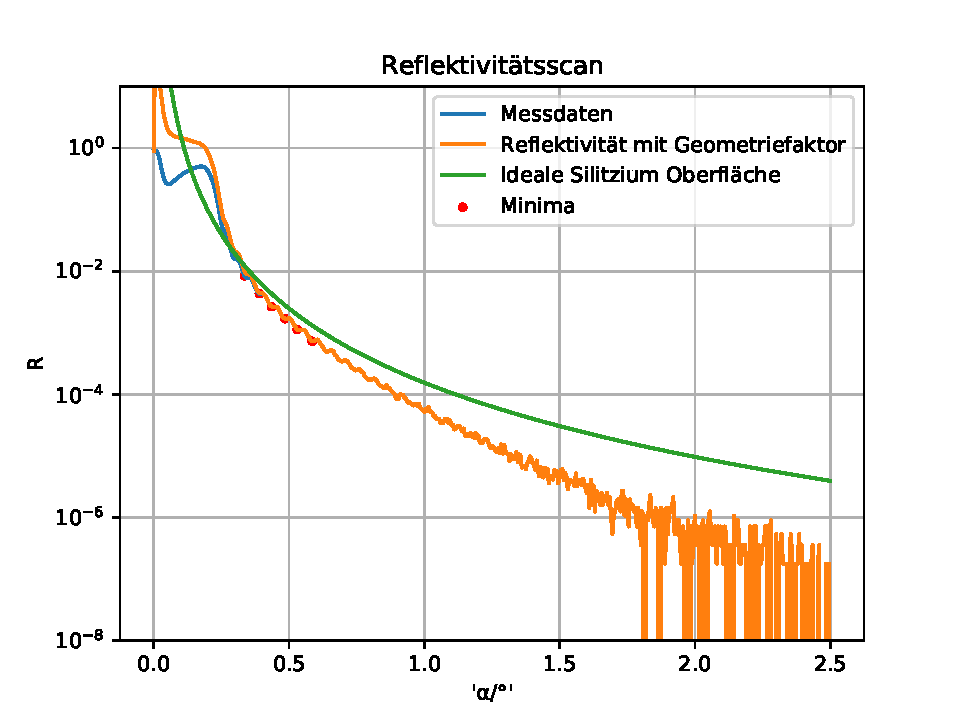
\includegraphics[width = 1\textwidth]{Auswertung/Graphen/Reflektivitaetsscan.pdf}
    \caption{Messwerte des Reflexivitätsscans mit und ohne Korrektur durch den Geometriefaktor im Vergleich zur idealen Siliziumoberfläche, sowie die Minima der Kiessig-Oszillationen.}
    \label{fig:ref}
\end{figure}
Dabei ist zu beachten das neben dem Winkel die Reflektivität
\begin{equation*}
    R = \frac{I}{5\cdot I_{max}} 
\end{equation*}
aufgetragen wird.
Zusätzlich ist auch die Korrektur durch den Geometriefaktor aufgetragen,
der berücksichtigt,
dass erst ab einem gewissen Winkel der komplette Strahl die Oberfläche trifft.
Ebenso ist die Reflektivität einer glatten Silizium Oberfläche dargestellt,
die mittels
\begin{equation}
    R = \left(\frac{\alpha_c}{2\alpha_i}\right)^4
\end{equation}
berechnet wird. 
Der Literaturwert für den kritischen Winkel $\alpha_c$ liegt für Silizium bei $\alpha_{Si} = 0,223°$ \cite{wert}

Die Schichtdicke lässt sich mithilfe der Kiessig-Oszillation aus der gemessenen Reflektivität bestimmen.
Dazu werden die auftretenden Minima untersucht und der gemittelte Abstand zwischen ihnen bestimmt.
Relevant sind hierbei nur die deutlichen ersten Minima (vg. Tabelle´v\ref{tab:scan})
\begin{table}
    \centering
    \caption{Ermittelte deutliche Minima des Rockingscans} 
    \label{tab:scan}
    \begin{tabular}{ r | r}
        \hline			
        Winkel [$\alpha/^°$] & R \\
        \hline
        0.345  & 0.0077  \\
        0.39   & 0.0043  \\
        0.435  & 0.0027  \\
        0.485  & 0.0016  \\
        0.53   & 0.0011  \\
        0.585  & 0.0007  \\
    \hline  
  \end{tabular}
\end{table}

Der gemittelte Abstand dieser ergibt sich zu
\begin{equation}
    \Delta\alpha = (0.045 \pm 0,003)°.
\end{equation}
Mittels der Gleichung
\begin{equation}
    d = \frac{\lambda}{2\Delta\alpha_i}
\end{equation}
ergibt sich daraus eine Schichtdicke von
\begin{equation}
    (882,4 \pm 20) \, \text{\AA}.
\end{equation}
Dabei ist zu beachten, 
dass die gemessenen Winkel im Bogenmaß eingesetzt werden,
da ansonsten die Dimensionen nicht stimmen.

\subsection{Parratt-Algorithmus}

Mit hilfe des Parratt-Algorithmus lässt sich das Dispersionsprofil bestimmen,
wie auch die kritischen Winkel von Silizium und Polystrol.
Verwendet werden dazu die modifizierten Fresnelkoeffizienten.
Das Modell funktioniert mit zwei Schichten, eine aus Polystrol und eine aus Silizium.
Die Umgebungsluft wird als eine Schicht mit der Schichtdicke und der Disperison von $d = \delta = 0$ angenommen.
Die entsprechende Kurve ist in Abbildung \ref{fig:parratt} dargestellt.
\begin{figure}[h]
    \centering
    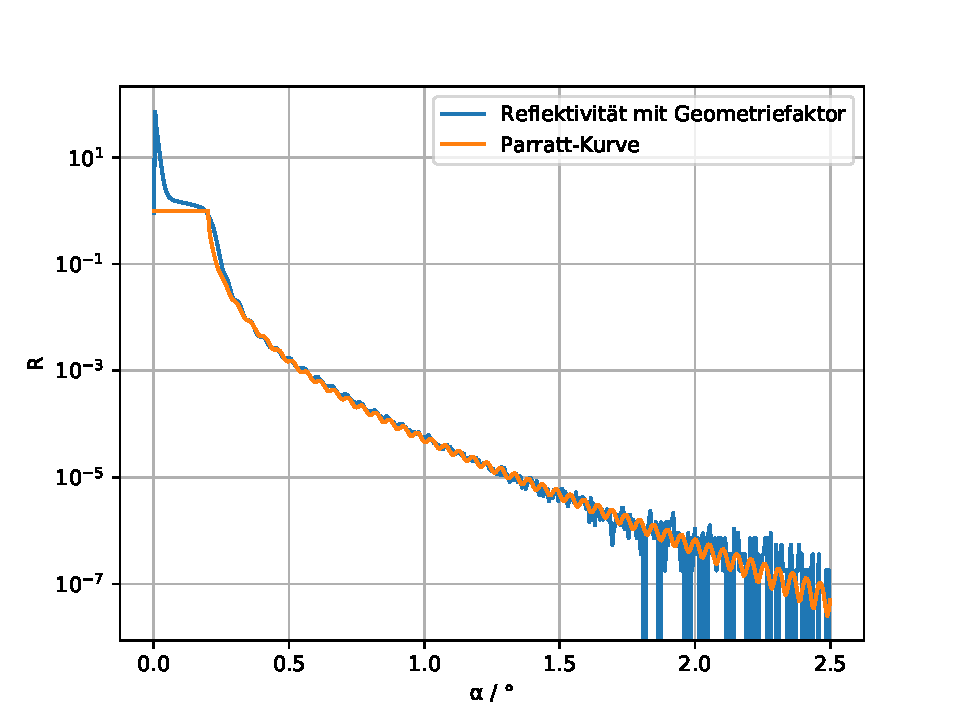
\includegraphics[width = 1\textwidth]{Auswertung/Graphen/Parrat_Algorthmus.pdf}
    \caption{Die Parrat-Kurve im Vergleich zur gemessenen Reflexivität.}
    \label{fig:parratt}
\end{figure}
Mittels der Gleichung \eqref{eq:krit} lässt sich der kritische Winkel der beiden Schichten jeweils bestimmen als:
\begin{align}
    \alpha_{Pol} &= 0,068^° \\
    \alpha_{Si}  &= 0,214^°
\end{align}
Die Parameter der Schichtdicke $d_2$, der Dispersion $\delta$ und der Rauigkeit $\sigma$ müssen per Hand so bestimmt werden,
dass die Parrattkurve eine möglichst große Übereinstimmung zeigt.
Demnachzufolge sind:
\begin{align*} 
    d_2 &=  860 \, \text{\AA} \\
    \delta_{Poly} &= 0.3\cdot 10^{-6}\\
    \delta_{Si} &= 6.3\cdot 10^{-6}\\
    \sigma_{Poly} &=  1.0\cdot 10^{-10} \, \mathrm{m}\\
    \sigma_{Si} &=  5.5\cdot 10^{-10} \, \mathrm{m}
\end{align*}
